SDIPI signifie "Swiss Digital Identity and Privacy Institute", pouvant se traduire par "Institut Suisse de l'Identité Digitale et de la Vie Privée". Il s'agit d'une association crée dans le but initial de soutenir le projet dans sa visibilité et dans sa légitimité, mais qui aspire à des objectifs généraux plus larges : Le but est de sensibiliser le public Suisse à la manière dont ses informations privées sont  enregistrées, traitées, croisées et utilisées.

\begin{figure}[h]
	\centering
	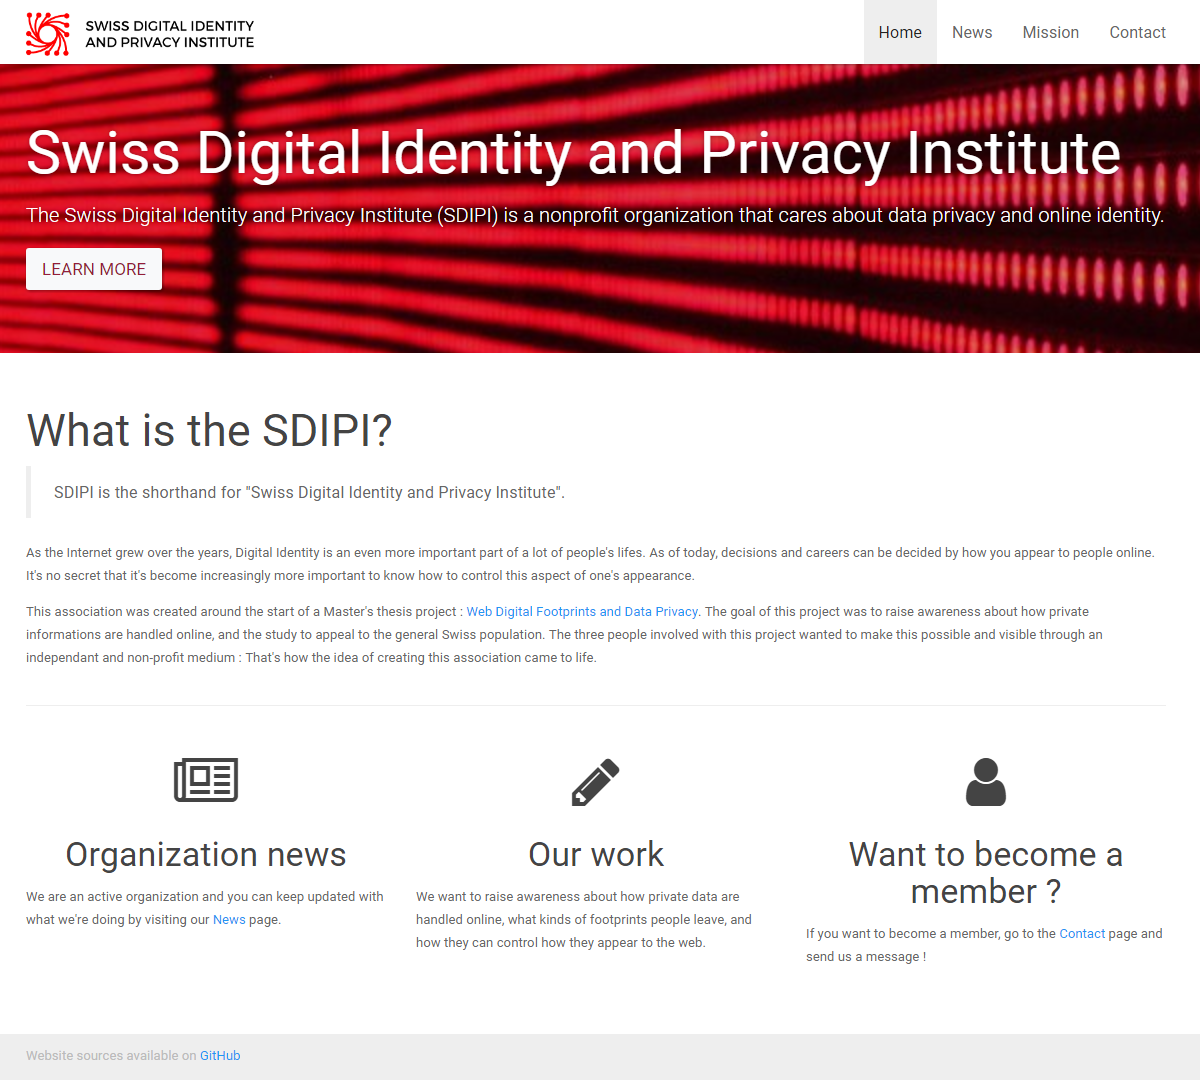
\includegraphics[width=1\textwidth]{images/design/sdipi_home}
	\caption{Page d'accueil du site web \url{https://sdipi.ch}.}
	\label{a-sdipi}
\end{figure}